%%%%%%%%%%%%%%
%%% DESIGN %%%
%%%%%%%%%%%%%%

\chapter{Design}
\label{design}

This chapter reports the design process for building a composite device that integrates smartphones to tabletops and provides a spontaneous user interaction.

A user-centered design approach was followed, in the purpose of understanding the system's context of use, and identifying the interaction techniques that would make for an intuitive application.
This process was supported by methodological tools described in Designing Interactive Systems \citep{Benyon:2010}.
Brainstorming, scenarios, storyboards and low-fidelity prototypes were used, and a study involving end users was carried out, the results of which informed the final design.

\begin{figure}[htb]
  \centering
    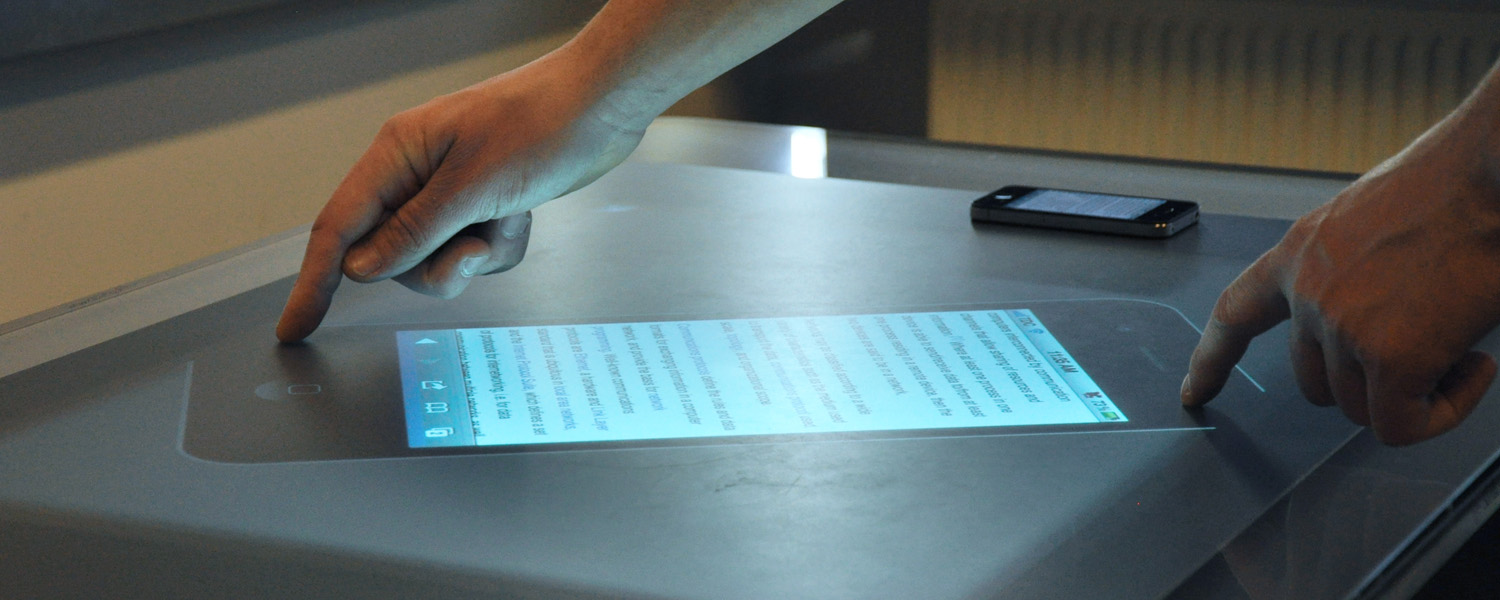
\includegraphics[width=0.8\textwidth]{images/tide314}
    \caption{The TIDE prototype.}
    \label{fig:tideHands}
\end{figure}

The focus of the design was on learnability and ease of use.
The goal was to build an intuitive system, i.e.\ a system that users understand without conscious reasoning.

To reach this goal, the design principle of conceptual consistency, as defined by \cite{Benyon:2010}, was used.
In this particular case, consistency was used in relation to two important aspects.
First; given that all the users of the system are smartphone users, the final system should provide a user experience that is as consistent possible with the smartphone experience.
Second; the user interaction should be consistent with the implications that the devices' form have on the user's expectations.
In particular, the interaction should be consistent with the form of the table, e.g.\ various objects could be placed on the tabletop during an application session.
\\
\linebreak
It was decided to limit the focus of this work to one interaction metaphor: \emph{UI replication}.
This metaphor was chosen among the different possibilities enumerated in Chapter~\ref{relatedwork}, for the following reasons.
Firstly, UI replication allows for a strong consistency between the experience on the smartphone and the experience on the tabletop.
Secondly, UI replication implies that the smartphone's application logic stays unchanged, and allows for the development effort to be focused on the tabletop.
Thirdly, for the same reason as mentioned above, the implementation can be made to support different types of smartphones.

Thus, the system is designed to present the user with a mirrored image of the smartphone UI on the tabletop.
This is referred to as the \emph{replicated UI}.
It is interactive, relaying touch input and graphical output between the smartphone and the tabletop.
The replicated UI is controlled by the \emph{surface UI}.
The surface UI consists of elements that allow for manipulation of the replicated UI on the tabletop.
\\
\linebreak
An analysis of the context of use is presented in section~\ref{sec:context}, from which solution requirements are derived in section~\ref{sec:requirements}.
Section~\ref{sec:interaction} describes the generation of design options for the surface UI and their evaluation.
The final design of the TIDE prototype is presented in section~\ref{sec:design}.

\section{Understanding the application context}
\label{sec:context}

Some initial design constraints are already known; the system integrates smartphones to tabletops, and the system uses UI replication to extend the smartphone UI to the tabletop.
%Figure \ref{fig:useCase} describes the primary use case.
In this section, additional design constraints are derived from an analysis of the devices, and the context of use is investigated through the use of scenarios.

%\begin{figure}[htb]
%  \centering
%    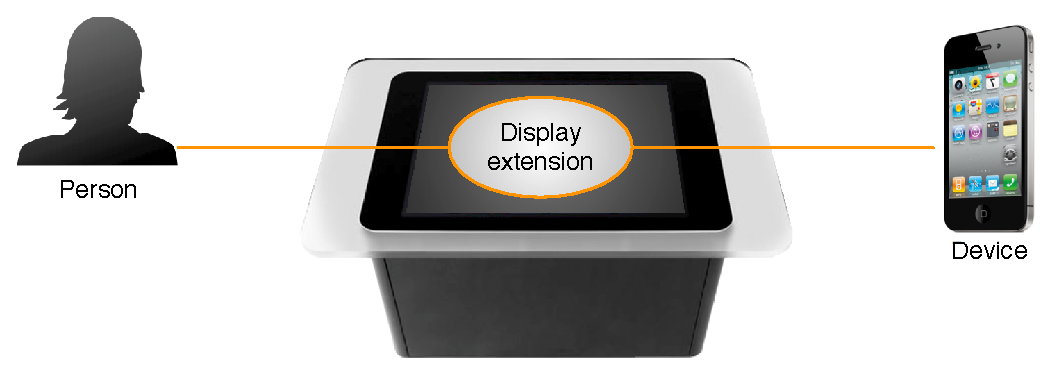
\includegraphics[width=0.9\textwidth]{images/useCase}
%    \caption{Main use case.}
%    \label{fig:useCase}
%\end{figure}

%Most users own a computing device with personal data and applications that are tailored to their needs.
%Those personal devices are becoming smaller and more mobile, with devices such as tablet and handheld computers.
%In many cases, the display size of the personal device is a limitation in terms of graphical input and output, and has a negative influence on the user experience.
%One of the main characteristics of tabletops, however, is that they have superior graphical I/O capabilities.
%This project focuses on situations where a tabletop can be used as a display extension to the personal device, thus enhancing the user experience.

\subsection{The devices}

The basic characteristics of the devices have concrete implications on the system design.

\subsubsection{A tabletop is\ldots}

\begin{description}

\item[\ldots a computer.]
The tabletop provides computing resources such as processing power, memory and connectivity; as well as an operating system that supports software applications.

\item[\ldots a table.] 
Its physical form comprises a horizontal surface that is commonly used to support various material objects.
A table is used for various activities, such as studying, eating, playing games, holding meetings, etc.
It can be approached from all angles, encouraging face-to-face interaction between multiple users.
%The system should therefore support simultaneous users, and handle limited space availability.

\item[\ldots a situated device.] 
It usually sits at a location, and is not moved often.
It can be expected to have dedicated power supply and network connection.
Users approach it to use it, and leave when they are finished.
Thus, the interaction flow is likely to be interrupted, taking the form of short successive sessions.
The nature of the location has an impact on the user interaction, and should be considered.
Examples are a conference room, a public lobby, a mall, an individual office, a living room in a family house, etc.
%The main implication is that tabletops seem to naturally fit in public spaces, where they are shared among multiple users.
%This tendency is accentuated by the price factor, that makes a private person not likely to buy such a device for private use.
%The system should handle public use, characterized by short anonymous sessions and an often interrupted interaction flow.

\item[\ldots a shared device.] 
When located in a public space, the tabletop is shared among multiple users.
Depending on the context and the relationship between the users (friends, colleagues, strangers, etc), the level of trust varies.

\item[\ldots an interactive surface.] 
It typically offers a large graphical output, and a range of input techniques that allow for user interaction.
Most tabletops support multitouch-based input.
%This introduces a new kind of interaction model, more intuitive, that the system should be based upon.
Some tabletop models support computer-vision techniques that allow for the integration of tangible objects to the interaction.
%This project reports on the possibilities to use a personal device as a tangible control integrated to the tabletop.

\end{description}

\subsubsection{A smartphone is\ldots}

\begin{description}

\item[\ldots a computer.] 
It provides the computing resources necessary to allow a user to connect, store personal data and install/use applications.
It runs on a mobile operating system that supports software applications.
%The system should allow the user to access his/her applications and personal data.

\item[\ldots a small device.] 
It is designed to fit in a pocket.
Smartphones are typically less than 5'' high, 3'' wide, and 0,6'' deep.
The small form factor implies some hardware limitations: resources such as battery life and processing power can not be taken for granted.
%However, the small form factor implies a suboptimal graphical user experience.
%The system should try to improve this, by offering superior IO resources.

\item[\ldots a mobile device.]
It is carried around by users at all times.
It is mostly used as a wireless device, across networks, implying a level of instability in the connectivity.
%The system should be developed with those concerns in mind.

\item[\ldots an interactive device.]
Modern smartphones typically include touch-based screens, as well as physical buttons, to allow user interaction.
%making them naturally suitable for display extension on a tabletop.
%The physical buttons implement strategic functions that the system should support.

\end{description}

\subsection{The situations}
\label{sec:scenarios}

Understanding the situations in which the system will be used is a step towards the elicitation of solution requirements.
The scenarios that were used to help define those situations are included in appendix \ref{scenarios}.

\begin{figure}[htb]
  \centering
    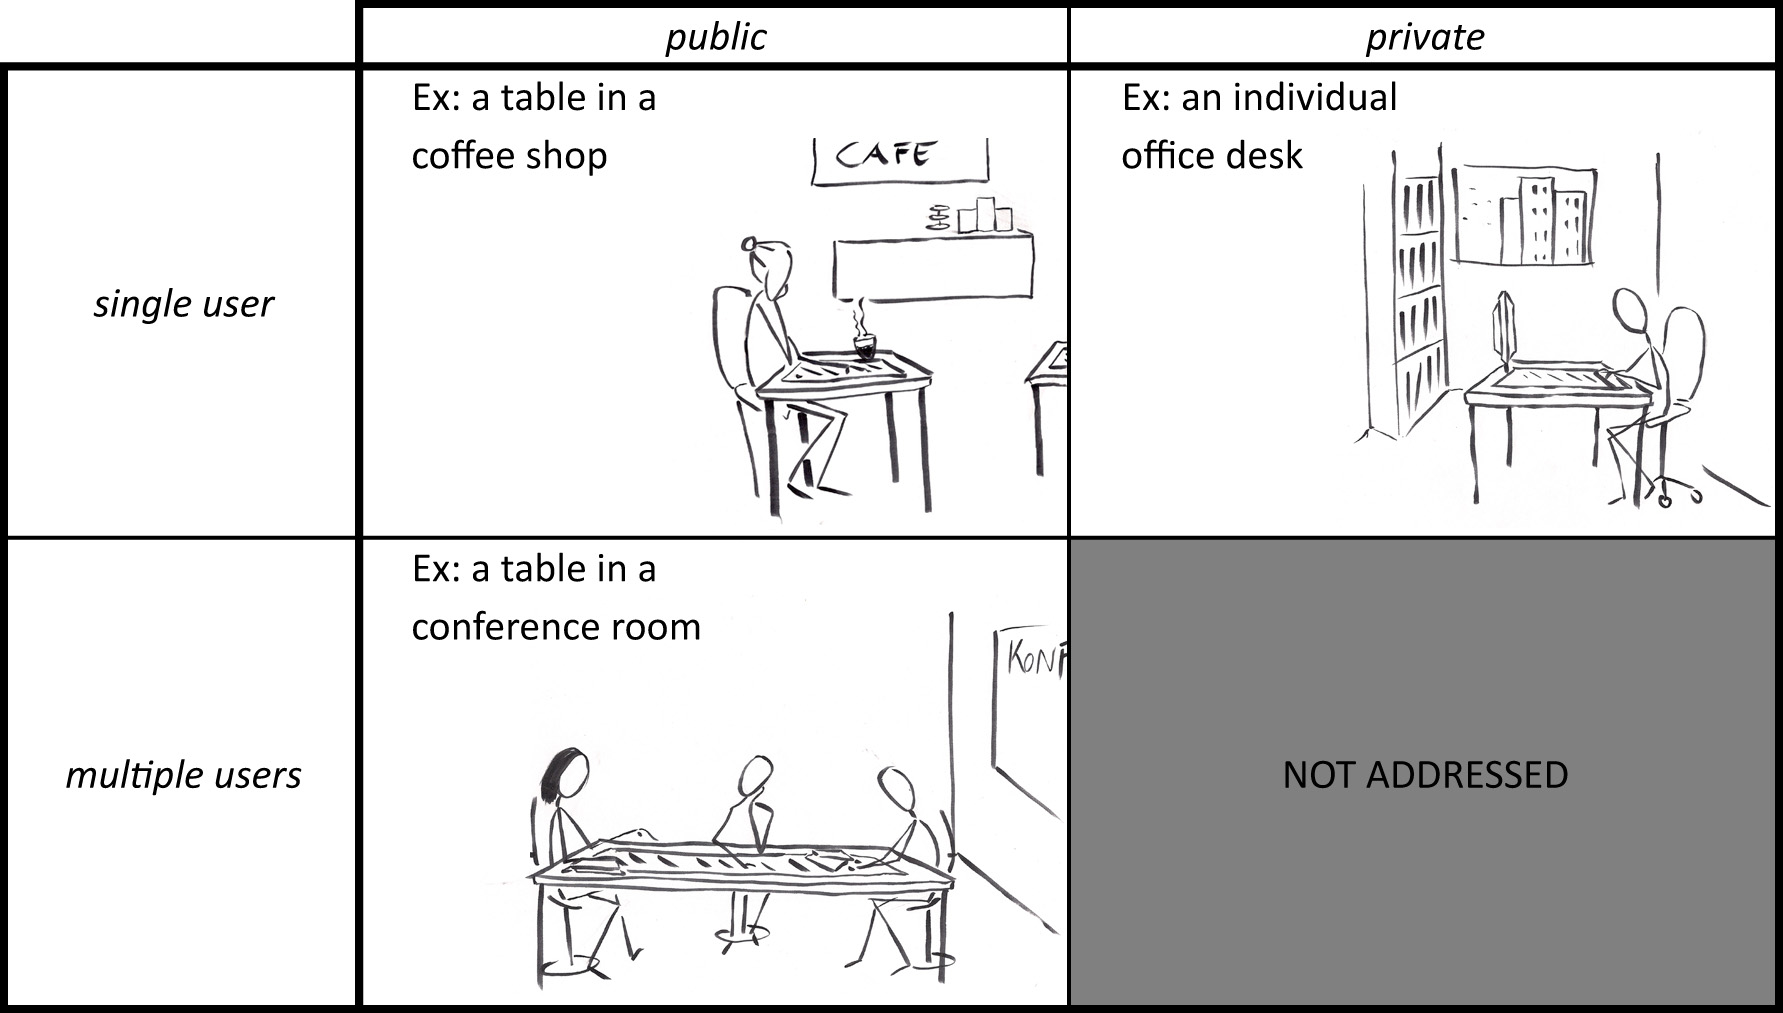
\includegraphics[width=0.8\textwidth]{images/marietable}
    \caption{The different situations in which the system can be used.}
    \label{fig:scenarios}
\end{figure}

As shown in figure~\ref{fig:scenarios}, the scenario depends on the level of privacy of the location (public/private) and the amount of involved users (single/multiple).

There are four combinations, however the situation with multiple users in a private location is not addressed here, for the reason that the tabletop cannot be considered private if multiple users are present.

\subsubsection{Single user with a public tabletop}

This situation was derived from a scenario involving a person sitting alone at an interactive table in a coffee shop.

In this environment, the motivation for using the system is an activity that involves graphically intense content, such as 
internet browsing, reading, consulting a map, etc.
To start using the system, the user pairs the smartphone with the tabletop.
The process is quick and easy, but not completely automatic.
The user must explicitly allow the connection to be established.
The user does not usually need cables to use the smartphone.
Ideally, the connection with the tabletop is handled wirelessly.
The replicated UI appears on the tabletop, and the user starts interacting with the application.
The surface UI provides the user with features to manipulate the replicated UI, in particular: dragging, rotating and resizing.
Via the surface UI, the user can minimize and hide the replicated UI, as well as exit the application.

The smartphone itself is involved in the interaction.
Placing it on the table triggers the pairing process.
During the interaction, the replicated UI is collocated with the device, and moves together with it.
Lifting the smartphone off the table ends the connection.

%It should be possible for the user to wirelessly pair his/her personal device with a public tabletop computer.
%This implies that the devices are both connected to the local wireless networks, that they are able to detect each other and discover each other's identity on the network.
%It would not be safe to establish this connection automatically in a public space.
%Therefore, dialogs should be used both on the mobile device and on the tabletop to gather user input.
%The UI of the mobile device should be transferred to the interactive surface as graphical output, and this transferred display should be able to accept touch input to be forwarded back to the device.
%The transferred display should be contained in an application window, and this window should be manipulable (drag, resize, rotate, minimize, hide, ..).

%The application window should react to the state of the interactive surface.
%An example of this is that the application window should turn inactive if it is obstructed by an object on the table.

%\begin{itemize}
%\item{the mobile device is automatically detected by the tabletop}
%\item{dialog windows are displayed on both devices}
%\item{the wireless connection is automatic}
%\item{the mobile device UI is transferred to the surface.}
%\item{the transferred UI can be resized, rotated and moved on the surface}
%\item{the transferred UI goes inactive when objects obstruct it}
%\item{user input is forwarded to the mobile device}
%\item{the transferred UI can be minimized and restored}
%\item{the application can be exited by lifting the mobile device off the table.}
%\end{itemize}

\subsubsection{Multiple users with a public tabletop}

This situation was derived from a scenario involving some work colleagues having a meeting in a conference room, equipped with an interactive tabletop.
It can be argumented that such an environment is only partly public, being only accessible to the people working in the company.
However, in an effort to produce a design as generic as possible, and for the sake of simplicity, the tabletop is here considered a public device.

The motivation to use the system in this context is to view, comment and possibly edit digital data in a collaborative meeting.

Multiple users might want to connect their smartphones to the system simultaneously.
%This implies that the implementation should support parallel connections and simultaneous use.
Due to the lack of space on the table, the users remove their devices, but keep the replicated UI active on the tabletop.

%Mobile computing devices come in many forms, and ideally the system should support all of them.
%Devices vary in terms of software and hardware specifications.
%Some parameters that are especially important here are the programming platform, as well as the display resolution.

\subsubsection{Single user with a private tabletop}

This situation was derived from a scenario involving a user whose office desk is a tabletop.

The motivation for using the system is that it is a tool that the user interacts with daily, to support various activities related to the work routine.

The tabletop being private, can be configured to provide extended functionalities.
Examples of extended functionalities are: the pairing procedure can be made automatic and data can be shared between the devices.

%Some suggested functionalities are:
%\begin{itemize}
%\item automatic launch of the display extension application
%\item push application widgets from the extended display to the tabletop
%\item share data between the personal device and the tabletop
%\end{itemize}

\section{Solution requirements}
\label{sec:requirements}

Based on the analysis of the application context, the following requirements were derived.
Only the requirements that were relevant to the problem at hand were included.
They are divided into four categories, that each correspond to a different aspect of the system: the pairing procedure, the UI replication, the surface UI and the use of the smartphone as tangible UI.

However, the following fundamental requirement is not attached to any category, as it relates to several system aspects:
\begin{enumerate}[{R}-1]
\item \emph{The system should support multiple simultaneous devices.}
\end{enumerate}

\subsection{Pairing}

The pairing procedure is responsible for device discovery and connection.
It should fulfill the following requirements:

\label{RA}
\begin{enumerate}[{RA}-1]
\item Pairing the devices should be easy and quick.
\item Discovery between the devices should be automatic.
\item Establishing the connection should require explicit confirmation from the user.
%\item Automatic pairing should be an available option in trusted setups.
\item Closing the application should be easy and quick.
\end{enumerate}

%Connecting a personal device to a tabletop should be a quick and easy process.
%The system should include a detection mechanism that would allow the devices to become aware of each other, as well as a discovery protocol to gather the information necessary to the pairing, such as a Network IP.
%The connection should be wireless to guarantee a smooth experience.
%However, a public tabletop should not be allowed to gather data from, let alone connect to, a personal device without the explicit consent of its owner.
%In the case of a trusted setup, it should be possible to bypass any explicit user input.
%Exiting the application and closing the connection should also be easy, allowing the system to handle short successive sessions.

\subsection{Tracking}

Tracking the location of the smartphone on the tabletop allows to link specific features to the physical device.
It should fulfill the following requirements:

\label{RB}
\begin{enumerate}[{RB}-1]
\item Placing the smartphone on the tabletop should trigger the pairing procedure.
\item The replicated UI should be collocated with the smartphone, i.e.\ the replicated UI should be seemingly linked to the device, and should move when the device is moved.
\item Lifting the smartphone off the table should trigger the application exit.
\item It should be possible to remove the smartphone, but keep the replicated UI active on the tabletop.
\end{enumerate}

%It is a natural thing to place an object on a table, and tabletops are designed to allow for the integration of physical artifacts.
%Therefore, it should be possible to use the personal device as a tangible UI.
%For example, it would seem obvious that placing the device on the tabletop would launch the pairing process, or that lifting it off would interrupt the connection.
%Furthermore, it should be possible to control the position of the display extension by sliding the personal device on the surface.

\subsection{Replicated UI}

The replicated UI is the interactive mirror image of the smartphone displayed on the tabletop.
It should fulfill the following requirements:

\label{RC}
\begin{enumerate}[{RC}-1]
\item The UI of the smartphone should be replicated on the tabletop.
\item The graphical output from the smartphone should be dynamically relayed to the replicated UI.
\item The touch-based input from the replicated UI should be dynamically relayed to the smartphone.
\item The responsiveness of the replicated UI should be under 1 second, for the user experience to be satisfactory.
\end{enumerate}

%At the core of the system is the display extension.
%The UI of the personal device should be transferred to the tabletop, allowing the user to interact with it in a natural way.
%Graphical output from the personal device should be forwarded to the tabletop, and touch-based input from the tabletop should be forwarded to the personal device.

\subsection{Surface UI}

The surface UI is the interface on the tabletop that controls the replicated UI.
It should fulfill the following requirements:

\label{RD}
\begin{enumerate}[{RD}-1]
\item The surface UI should be easy to use.
\item The surface UI should allow the user to manipulate the replicated UI, i.e.\ the user should be able to move, rotate and resize the replicated UI across the tabletop display.
\item The surface UI should allow the user to minimize and restore the replicated UI.
\item The surface UI should allow the user to hide the replicated UI.
\item The surface UI should allow the user to exit the application.
\item The surface UI should include controls that implement the functionalities provided by the physical buttons on the smartphone.
\end{enumerate}


%The user experience should be improved by using the display extension on the surface.
%Therefore, it is important to provide for a rich interaction.
%The transferred UI should be contained within a manipulable window on the tabletop.
%Specifically, the user should be able to move, rotate and resize the window; as well as minimize, hide and restore it.
%The system should include UI elements that implement the functions supported by the physical controls present on the personal device.
%Those elements and their function should be obvious to the user.
%
%%secondary features
%Modern smartphones include sensors that allow to switch the display orientation by tilting the device.
%This feature is strategic to certain applications, and should be implemented by the system.
%Obviously, tilting the tabletop is unfeasible, so another solution is necessary.
%
%As mentioned earlier, a tabletop's screen space would typically be shared among different applications and/or objects.
%Therefore, the system should handle limited screen space, and obstruction of the display extension.
%
%In a trusted setting, the user should have the possibility to push application widgets from the personal device to the tabletop, outside of the display extension, thus saving space on the latter.

\section{Designing the user interaction}
\label{sec:interaction}

This section focuses on the design of the surface UI, which comprises the UI elements that provide control over the replicated UI on the tabletop.
%As for the other system aspects, decisions were taken early in the process, that removed the need for a detailed design process.
The other system aspects did not require a detailed design process, for the following reasons.

First, it was decided that the pairing procedure should rely on already available solutions.
%as the focus of the thesis is not to contribute within this particular field.

Second, given that UI replication had already been decided upon, no design effort would be required for this system component.
%VNC was chosen as a protocol for UI replication, due to its stability and availability on most platforms.

Lastly, tracking the location of the smartphone is a technical requirement that does not require interaction design. %would only be used to trigger the pairing procedure.
\\
\linebreak
The input technique considered in the design of the surface UI is touch-based interaction.
The reason for this is that it is strongly consistent with the smartphone and tabletop experiences.
Both rely on touch-based interaction.
Moreover, the presence of other input peripherals cannot be expected, thus relying on touch-based input will ensure the system is usable in any setup.

The steps followed to design the surface UI were; (1) The generation of ideas, (2) The definition of \emph{interaction strategies} and (3) A study involving end-users to identify the interaction techniques that they find the most familiar.

%The pairing procedure does not introduce anything new to the field. There are known solutions to this challenge, which are described in section \ref{}.
%The remote UI replicates the UI of the personal device on the tabletop, and does not require any supplementary design.
%Using the personal device as a tangible UI for the display extension raises a series of design and implementation challenges. It is the opinion of the author that this research angle is promising, but it was decided to leave it out of the project for reasons of time constraints.
%\hfill\\

\subsection{Generating ideas}

The generation of ideas is an important part of the design process.
Benyon refers to it as envisionment \citep{Benyon:2010}, which he defines as the process of externalizing design thoughts.
The techniques that were used for this process are brainstorming, sketching, storyboarding and prototyping.

\subsubsection{Storyboards}

The scenarios mentioned in section~\ref{sec:scenarios} are used as a base for the making of storyboards.
Storyboarding helps finding the general flow of the system interaction.
It also gives a visual dimension to the definition of the different system features, and raises new design issues.
%Putting orally expressed ideas on the paper is often a first test of their validity.

As an example, several system features were described in the initial scenarios as being the result of a tap on a button.
When storyboarding, it became obvious that having too many UI buttons would crowd the user interface.
This caused consideration of other interaction techniques, such as touch gestures.
Similarly, the issue of the location and size of the replicated UI on application launch first became apparent on a storyboard.

\subsubsection{Low fidelity prototypes}

Paper prototypes were used to aid the process of generating and evaluating as many design solutions as possible.
Screenshots of the iPhone UI \citep{iphone} were printed in various sizes, and used on a normal table to simulate interaction with the replicated UI.
Figure \ref{paperProt} shows some prototypes and a working session.

\begin{figure}[htb]
  \centering
    \includegraphics[width=1\textwidth]{images/paperProtDouble}
  \caption{Working with low fidelity prototypes.}
  \label{paperProt}
\end{figure}

%\begin{figure}[h!]
%  \caption{Low fidelity prototypes.}
%  \centering
%    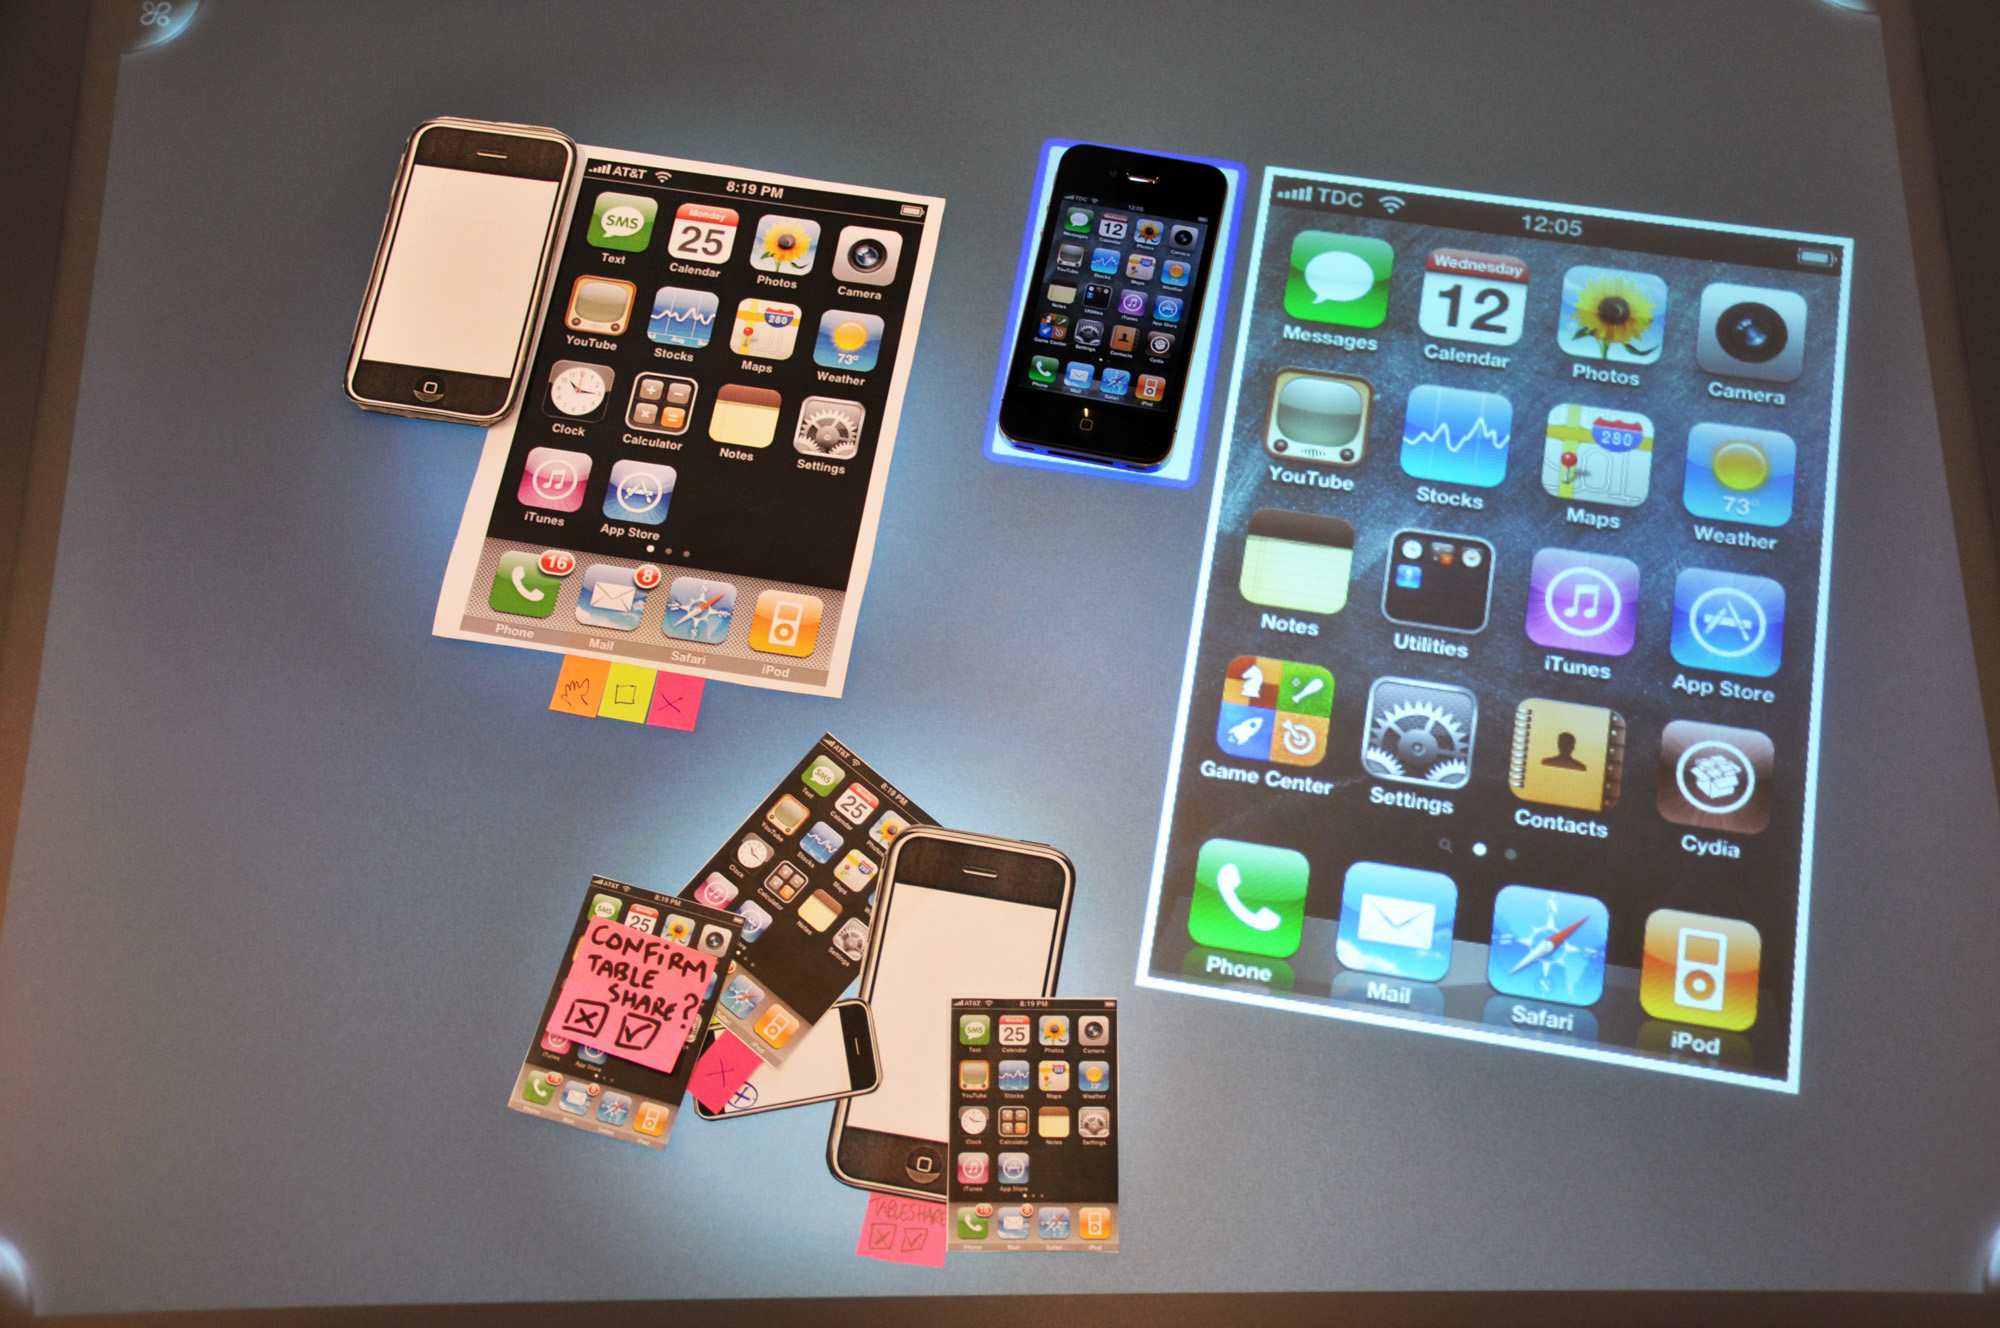
\includegraphics[width=0.8\textwidth]{images/paperprot2}
%\end{figure}

%\begin{figure}[h!]
%  \caption{Low fidelity prototypes.}
%  \centering
%    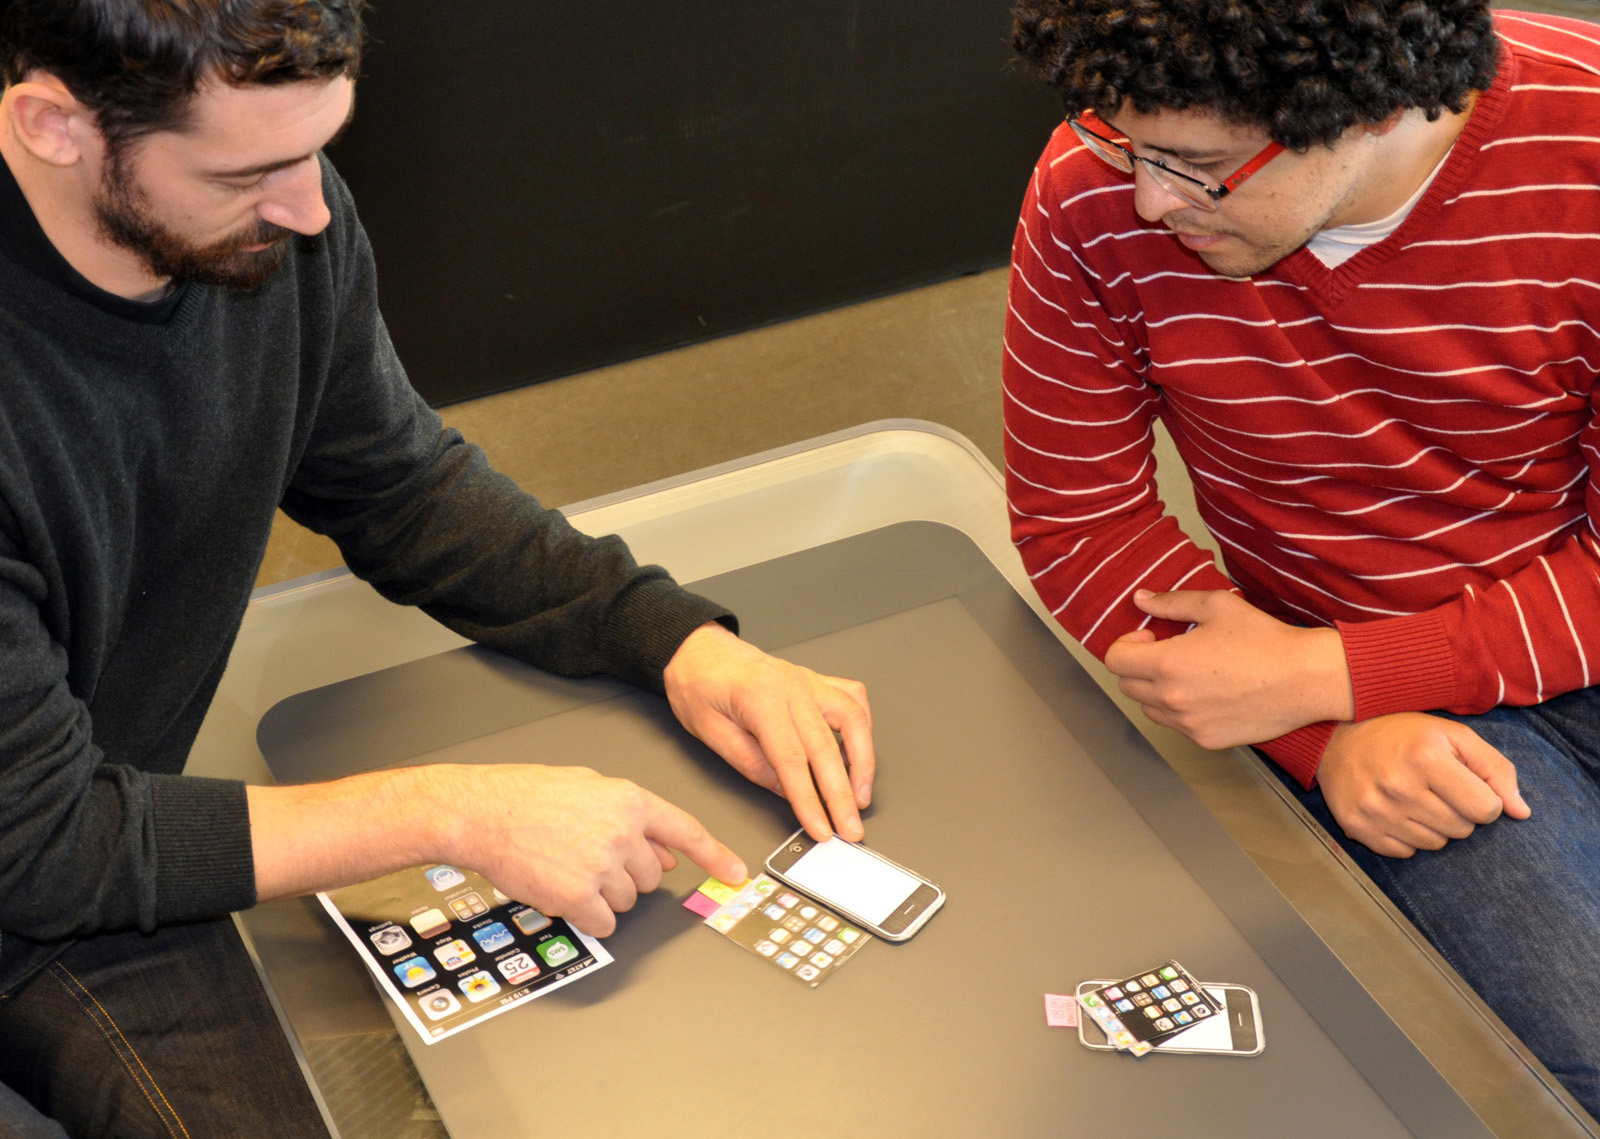
\includegraphics[width=0.8\textwidth]{images/paperprot3}
%\end{figure}

\subsection{Defining interaction strategies}
\label{sec:strategies}

The terms of \emph{actions} and \emph{commands} were used to refer to the different aspects of the user interaction.
They are inspired by the work done by Wobbrock et al. on defining hand gestures for interactive surfaces, \citep{Wobbrock:2009:gestures}.

A command is an \emph{effect} that the user wants to obtain, such as rotating a picture on a tabletop display.
An action is the \emph{cause} of an effect.
For example, using two fingers and performing a rotating gesture.
On a tabletop display, actions are typically hand gestures.

%Human computer interaction can be modeled as a simple cause-effect relationship.
%An action is a cause, a command is an effect, and together they form a single interaction between user and machine.

\subsubsection{Commands}

Based on the requirements formulated in section~\ref{sec:requirements} for the surface UI, the following six commands were identified.
They are the \emph{interaction primitives} for the surface UI, i.e.\ the commands that must be implemented by the surface UI, to allow the user full control of the replicated UI.

\begin{enumerate}
\item{\emph{Dragging} the replicated UI across the interactive surface.}
\item{\emph{Rotating} the replicated UI across the interactive surface.}
\item{\emph{Resizing} the replicated UI across the interactive surface.}
\item{\emph{Minimizing} the replicated UI, and restoring it.}
\item{\emph{Hiding} the content of the replicated UI.}
\item{\emph{Closing} the replicated UI.}
\end{enumerate}

Additionally, the surface UI should include controls that implement the functionalities provided by the physical buttons on the smartphone.

\subsubsection{Actions}

To invoke the commands that are defined above, a user needs to perform actions.
Various interaction techniques can be used to define these actions.
Figure~\ref{strategies} shows five \emph{interaction strategies} that were identified while working with paper prototypes.
Each strategy can be consistently implemented for all six interaction primitives.

\begin{figure}[htb]
\centering
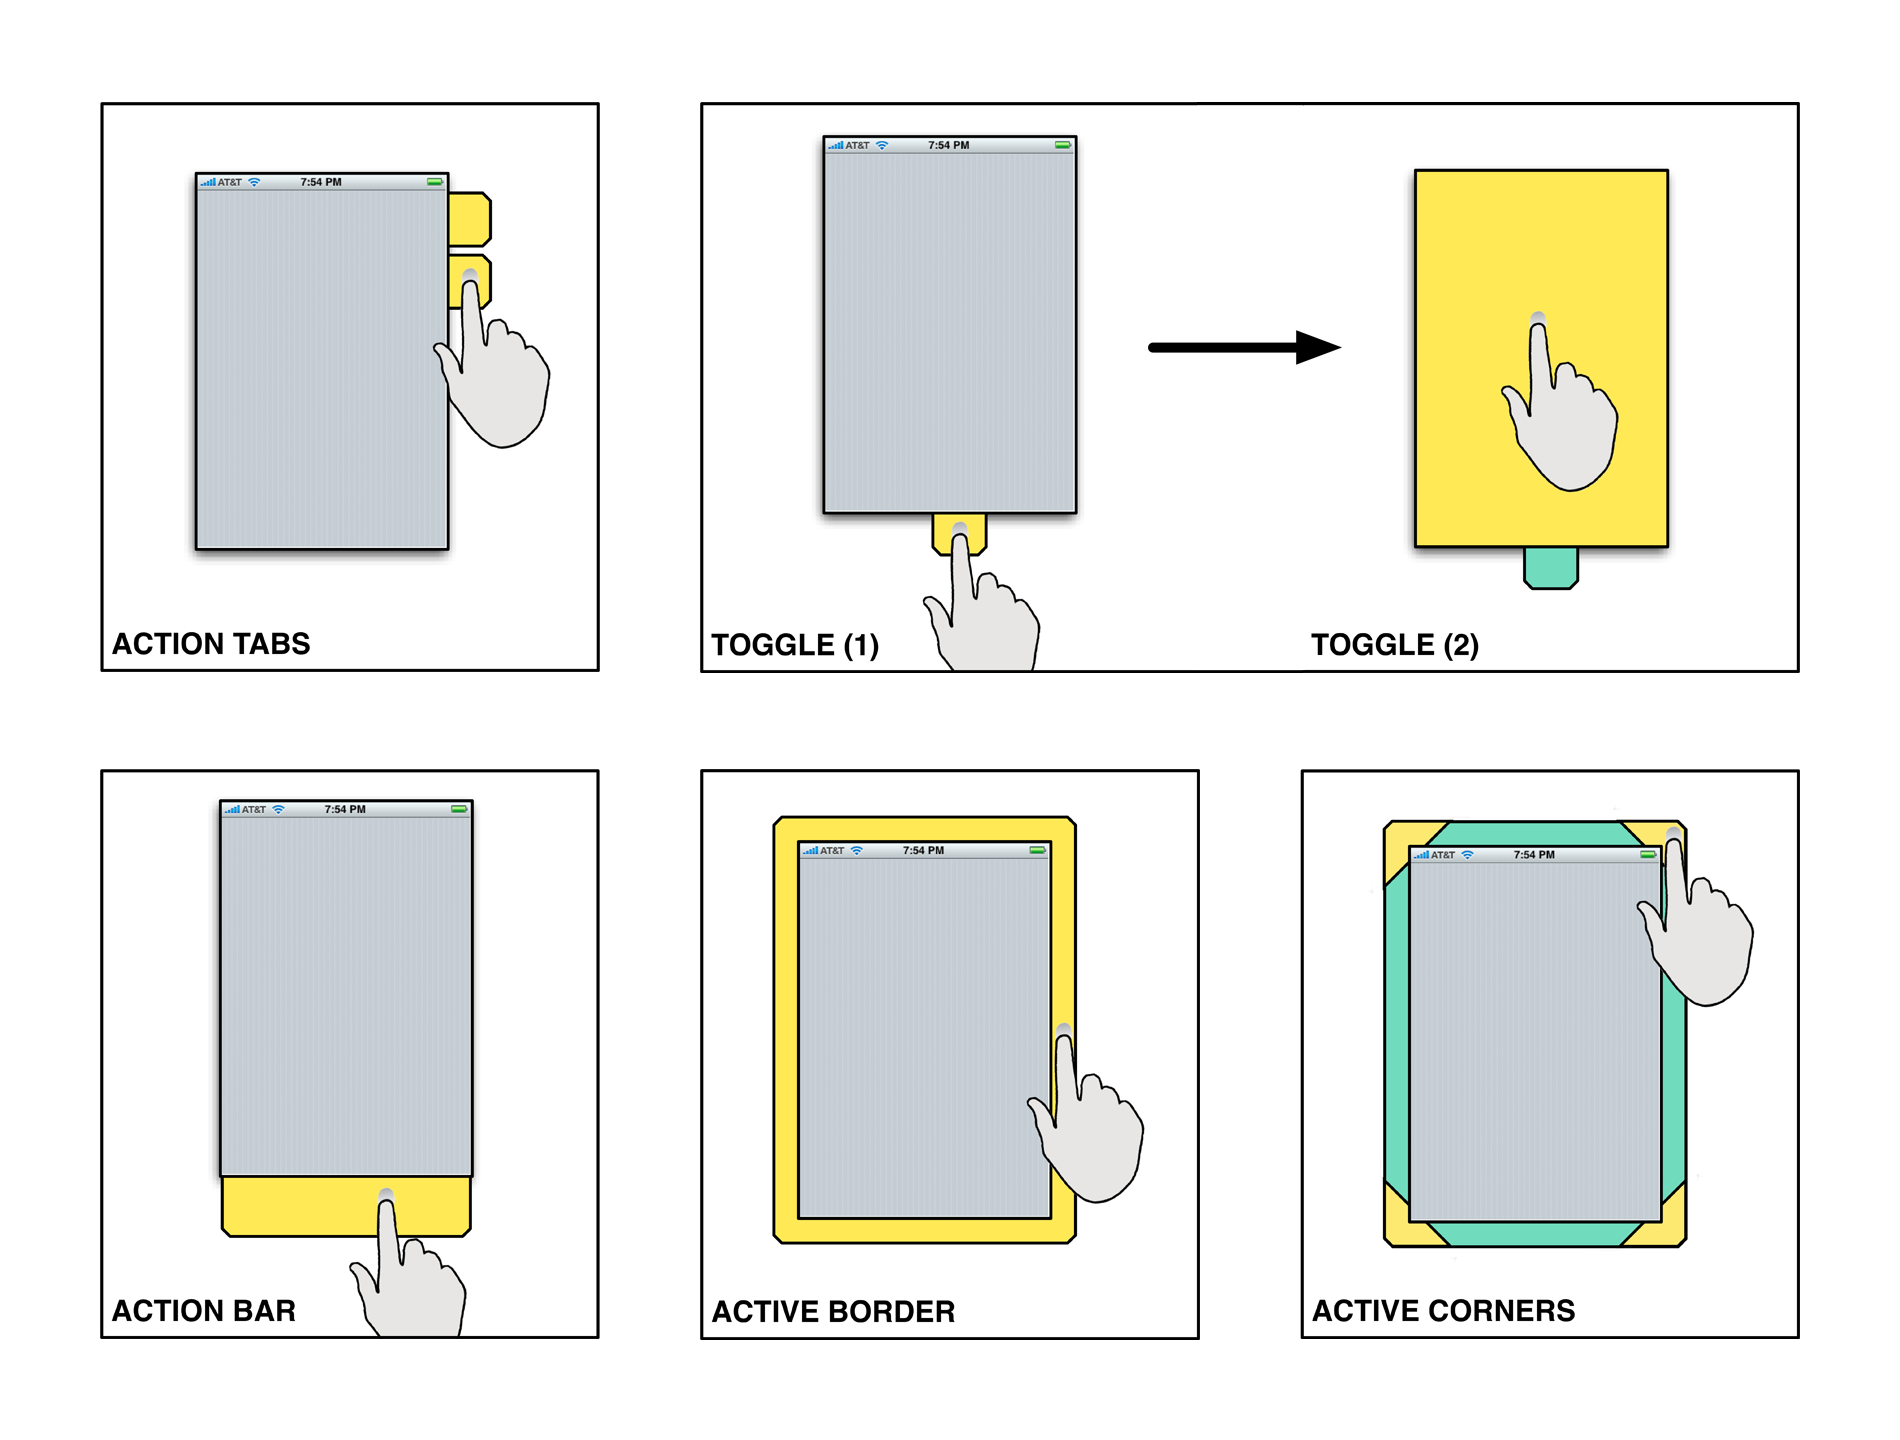
\includegraphics[width=1\linewidth]{images/strategies}
\caption{Interaction strategies.}
\label{strategies}
\end{figure}

\begin{enumerate}
\item{\emph{Action Tabs} are traditional buttons/tabs that implement functionalities.}
\item{The \emph{Action Bar} can be compared to a virtual touchpad, it includes a manipulation area and buttons.}
\item{\emph{Window Toggle} refers to using a switch to toggle the window between inactive and active states. In its inactive state, the window is made manipulable as a common digital picture.}
\item{The \emph{Active Border} is a digital frame around the application window used for manipulation.}
\item{\emph{Active Corners} is a strategy similar to Active Border, with the difference that the border's corners implement specific functionalities.}
\end{enumerate}

Beside these five interaction strategies, an additional category was used, that regrouped interaction techniques that did not correspond to any of the strategies.
This category is called \emph{Other}, and is discussed on page~\pageref{other}.

%\begin{figure}[ht]
%\begin{minipage}[b]{0.5\linewidth}
%\centering
%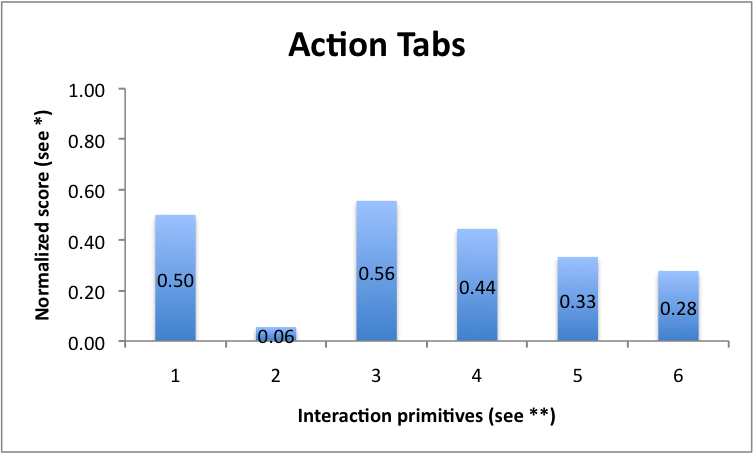
\includegraphics[width=0.6\linewidth]{images/strat1}
%\caption{action tabs prototype}
%\label{fig:strat1}
%\end{minipage}
%\hspace{0.5cm}
%\begin{minipage}[b]{0.5\linewidth}
%\centering
%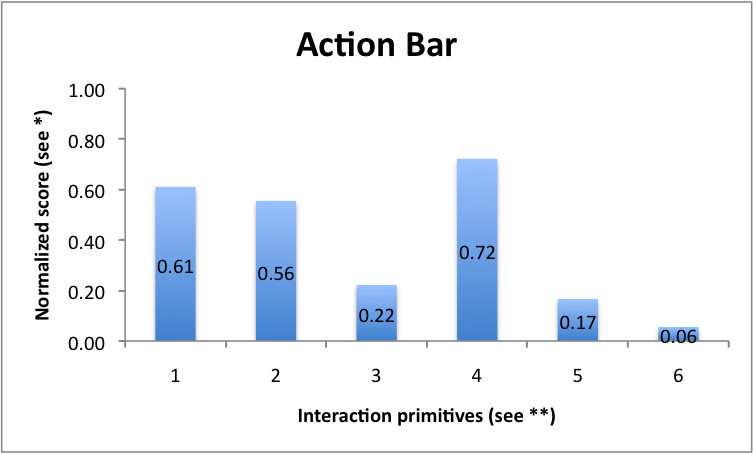
\includegraphics[width=0.6\linewidth]{images/strat2}
%\caption{action bar prototype}
%\label{fig:strat2}
%\end{minipage}
%\hfill\\
%\begin{minipage}[b]{0.5\linewidth}
%\centering
%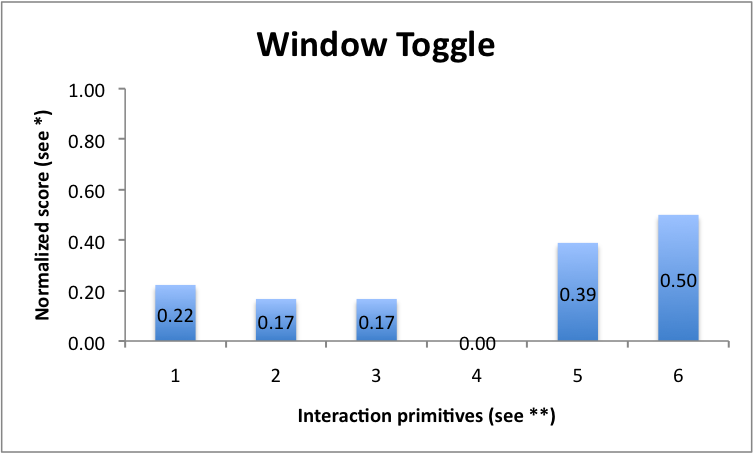
\includegraphics[width=0.6\linewidth]{images/strat3}
%\caption{active border prototype}
%\label{fig:strat3}
%\end{minipage}
%\hspace{0.5cm}
%\begin{minipage}[b]{0.5\linewidth}
%\centering
%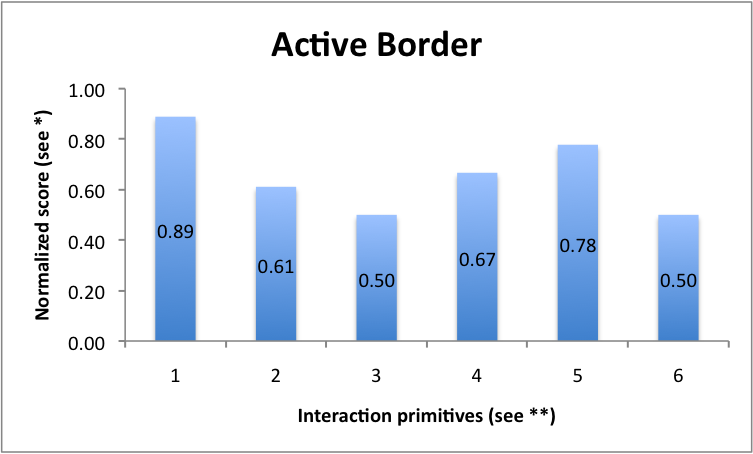
\includegraphics[width=0.6\linewidth]{images/strat4}
%\caption{active corners prototype}
%\label{fig:strat4}
%\end{minipage}
%\end{figure}

\subsection{Involving users}

To discover which of the defined interaction strategies were most intuitive, an experiment was carried out, that involved end users.
The experiment took the form of cooperative design sessions, where users engaged with low-fidelity prototypes of the system, in the aim of exploring and evaluating ideas.

The parameters of the experiment are the commands, also referred to as \emph{interaction primitives}, and the actions, also referred to as \emph{interaction strategies}, defined in section~\ref{sec:strategies}.

%The interaction primitives are central system features.
%For each primitive, the participants were asked to express an open-ended \emph{user suggestion}, then to \emph{rank} the interaction strategies.

\subsubsection{Experiment}

\begin{figure}[htb]
  \centering
    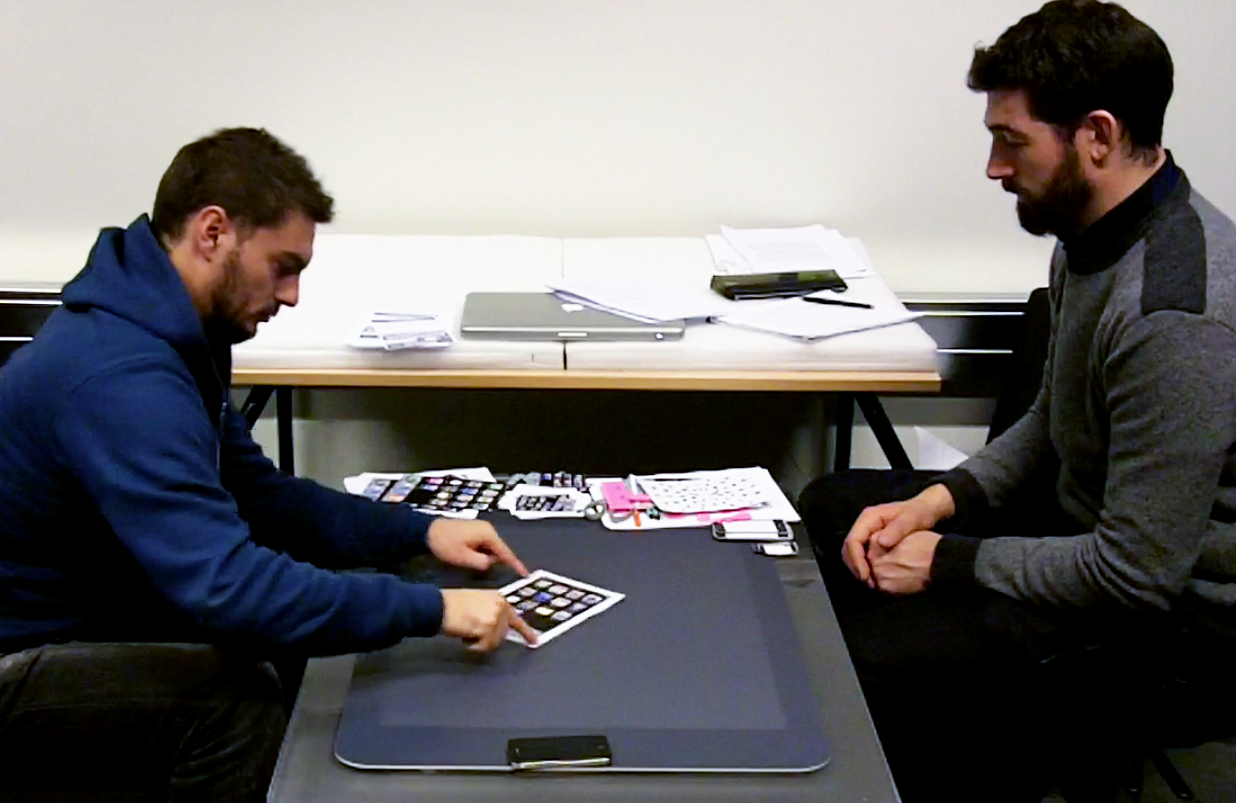
\includegraphics[width=0.8\textwidth]{images/studyScreenshot}
  \caption{Designing the surface UI with paper prototypes.}
  \label{fig:studyScreenshot}
\end{figure}

Twelve participants were recruited on a voluntary basis.
A session involved one participant and the designer, as shown in figure~\ref{fig:studyScreenshot}.
The participant sat next to the Microsoft Surface tabletop \citep{ms}, and was presented with an iPhone \citep{iphone}, but both devices were turned off.
On the tabletop were paper prototypes, that were to be used as representations of UI elements throughout the session.
The designer lead the experiment by reading instructions from a script (included in appendix~\ref{app:study}) and answering the participant's questions.
\\
\linebreak
As an introduction, the following things were explained to the participant:
\begin{itemize}
\item The purpose of the experiment
\item The purpose of the application
\item The tasks that the participant will perform
\item The principles of working with paper prototypes
\end{itemize}
\hfill
\linebreak
The session revolved around a task that the participant was asked to perform using the prototyped application.
The task was to write an email, and it required the user to go through six phases.
Each phase was dedicated to an interaction primitive, and they had the same structure, which is as follows:
\begin{enumerate}
\item The primitive was explained to the participant in terms of a command to the application.
\item The user was asked to express an open-ended suggestion, i.e.\ suggest an action that s/he would perform to obtain the desired effect, and to demonstrate the action using the prototypes,
\item The designer described action suggestions, that the user was asked to try out and rank by order of preference.
\end{enumerate}

%There is a seventh phase focusing on the pairing procedure.
%This phase occurs first and is meant as an example to the participant, describing the common structure.
%At the end of this phase, a slide animation is used to describe all six primitives to the user.

%For each command, there are six possible actions.
%However, it was decided that presenting a user with six options to rank would be overwhelming.
%The volunteers were therefore split into two groups, each evaluating a subset of the interaction strategies.
%The repartition is shown in table~\ref{groups}.
%
%\begin{figure}[htb]
%  \centering
%    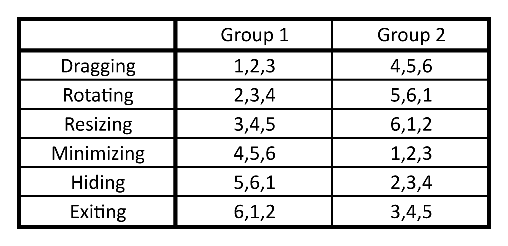
\includegraphics[scale=1]{images/groups}
%  \caption{The repartition of the evaluated interaction strategies between the two groups of participants. The strategies are 1)~Action Tabs 2)~Action Bar 3)~Window Toggle 4)~Active Border 5)~Active Corners 6)~Other.}
%  \label{groups}
%\end{figure}

\subsubsection{Data processing}

Participant answers were gathered in a form such as the one included in appendix~\ref{app:studyForm}.
The form is a matrix where an entry corresponds to a pair (primitive, strategy).
The entries contain the position from first (highest) to third (lowest), that was given by the user for using the suggested strategy for implementing the primitive.
After processing all answers, each entry contained six positions.
In order to obtain a numeric score for each entry, a weighted average was calculated.
A weight of 3 was given to a first position, a weight of 1 to a second position, and a weight of 0 to a third position.
Finally, the results were normalized to a [0-1] interval, where a 1 meant that the entry was awarded a first position by all participants, and a 0 meant that all participants ranked the entry third.
Figure~\ref{resultMatrix} summarizes the normalized scores, with colored cells containing values above 0.6.
This is considered a superior score, because it can only be obtained if half of the participants awarded the first position.
%The same results are presented in the form of charts in figure~\ref{primitives}.

The experiment data also included the user suggestions, gathered separately on paper.
User suggestions were not limited to one per primitive.
Thus, the processed data was a disparate list of suggestions that each had a counter variable indicating how many users independently expressed said suggestion.

\begin{figure}[htb]
  \centering
    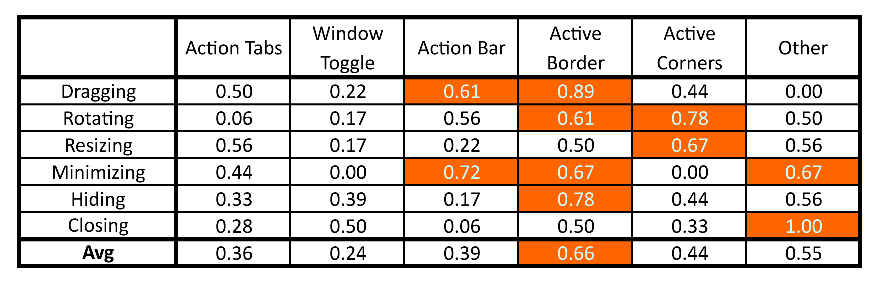
\includegraphics[scale=1]{images/resultMatrix}
  \caption{Normalized weighted average of the ranks given to each pair (primitive, strategy).}
  \label{resultMatrix}
\end{figure}

%\begin{figure}[h!]
%  \centering
%    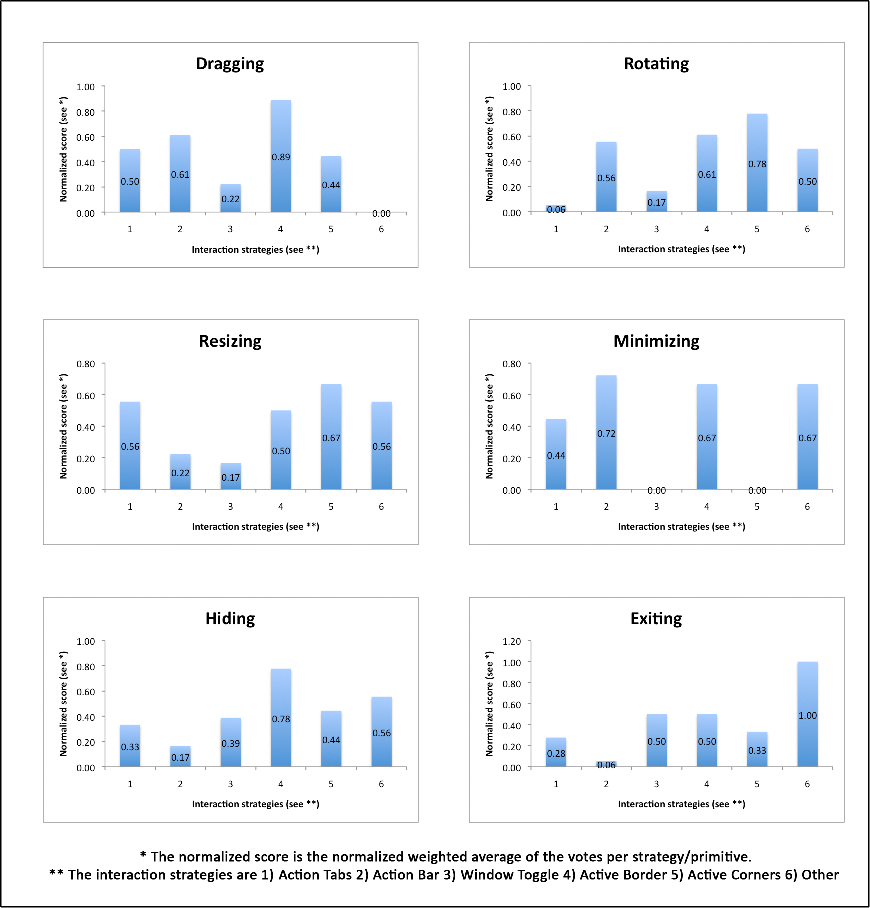
\includegraphics[width=1\textwidth]{images/primHistog}
%    \caption{The score of the different interaction strategies for each primitive.}
%	\label{primitives}    
%\end{figure}

\subsubsection{Result Analysis}

It is possible to divide the primitives into two groups.
The first half---dragging, rotating, resizing---have a concrete visual signification.
The second half---minimizing, hiding, closing---are more abstract.

For the first three primitives, there is a strong coherence in the choice of the participants.
The favored strategies are the active border, the action bar and active corners.
All three require the user to interact with an area directly around the window in order to manipulate it and modify its position, orientation or size.
This interaction technique is similar to the current standard for manipulating pictures on interactive screens.
However in the present case, the replicated UI is logically avoided because of its role as IO relay between the tabletop and the smartphone.

For the last three primitives, the action bar and active border continue to score high, even though there is no apparent relation between the visual aspect of the strategy and the effect implied by the command.
To understand this, it is necessary to look at the actual suggestions.
The favored strategies for minimizing were double tapping on the action bar and double tapping on the active border.
For hiding, the favored strategy was double tapping on the active border.
It is thus obvious that it is the double tap that participants have a preference for, possibly because it is a common technique in many other application contexts, as well as a quick and easy one.
\\
\linebreak
\label{other} It is not possible to analyze the scores of the sixth category as a whole, as it does not represent a consistent strategy, but more a patchwork of various suggestions. They are:
\begin{enumerate}
\item Drag by holding a finger on a specific tab, and using another finger to tap a destination target to move the window.
\item Rotate by performing a one finger dragging gesture on a corner of the window.
\item Resize by pulling the window apart with both whole hands.
\item Minimize by dragging the window to the bottom of the surface.
\item Hide by placing and holding a full hand on the window.
\item Close by dragging the window to a specific location on the surface.
\end{enumerate}
Suggestions 4 and 6 are similar, and they are the only ones that scored above 0.6.
This suggests that moving the window off screen; is a natural way to remove focus from the application.
Interestingly, this correlates with the analysis of the user suggestions.

\subsubsection{User suggestions}

The user suggestions were multiple and heterogeneous, but data processing revealed a clear tendency in three situations.

In the case of dragging, half of the participants suggested using one or more fingers to touch within the replicated UI, and perform a drag gesture.
This is interesting, because it is an obvious conflict for the developer, i.e.\ any touch inside the replicated UI is forwarded to the smartphone, and logically can not be interpreted by the surface UI.
It must be noted that dragging was the first primitive, and it can therefore be assumed that the participants did not yet have a full understanding of the application concept.
However, this result shows what the ideal system should be able to do: interpret the intention of the user.

In the case of resizing, 8 out of 12 participants suggested grabbing the sides of the window with 2 fingers, and pulling the window apart to enlarge it.
This shows that the gesture is very intuitive, and that implementing it would definitely add to the usability of the system.

The third consensus was for minimizing, where 7 out of 12 participants suggested dragging the window offscreen (or to a specific location along the surface edge).
The same suggestion reoccurred for the primitives hiding and closing, though with less decisiveness.
Once again, it shows that the gesture is an intuitive one.
Moreover, it is consistent with the action of removing a real piece of paper from the center of a table.
%, and the act of minimizing, hiding or closing the display extension application.
%Moving the application out of focus seems like a good solution, and using a simple dragging gesture is a natural way of doing it.

\section{Final Design of TIDE}
\label{sec:design}

Based on the design analysis and in particular the feedback from the user experiment, the following design decisions were taken.
They relate to the requirements defined in section~\ref{sec:requirements}.
%In the continued effort to build an intuitive system, that provides a spontaneous user interaction, special focus was given to the design consistency, and in particular:
%\begin{itemize}
%\item The design should be consistent with itself. If the features are coherent, the user will be able to derive one from the other.
%\item The design should be consistent with the user background. In the present case, the user already has some expertise with a smartphone. Therefore, the design should be consistent with the touch-based interaction that is provided on most smartphones.
%\item The design should be consistent with the physicality of the devices. In particular, the tabletop form has implications on the user's expectations.
%\end{itemize}
\\
\linebreak
The requirement \emph{R-1 The system should support multiple simultaneous devices} will be fulfilled by the design decision:
\begin{enumerate}[{D}-1]
\item The system will be implemented with focus on loose coupling between the main application session classes and the objects handling individual devices, in order to support simultaneous devices, as shown in figure~\ref{fig:sq2phones}. 
\end{enumerate}
\begin{figure}[htb]
  \centering
    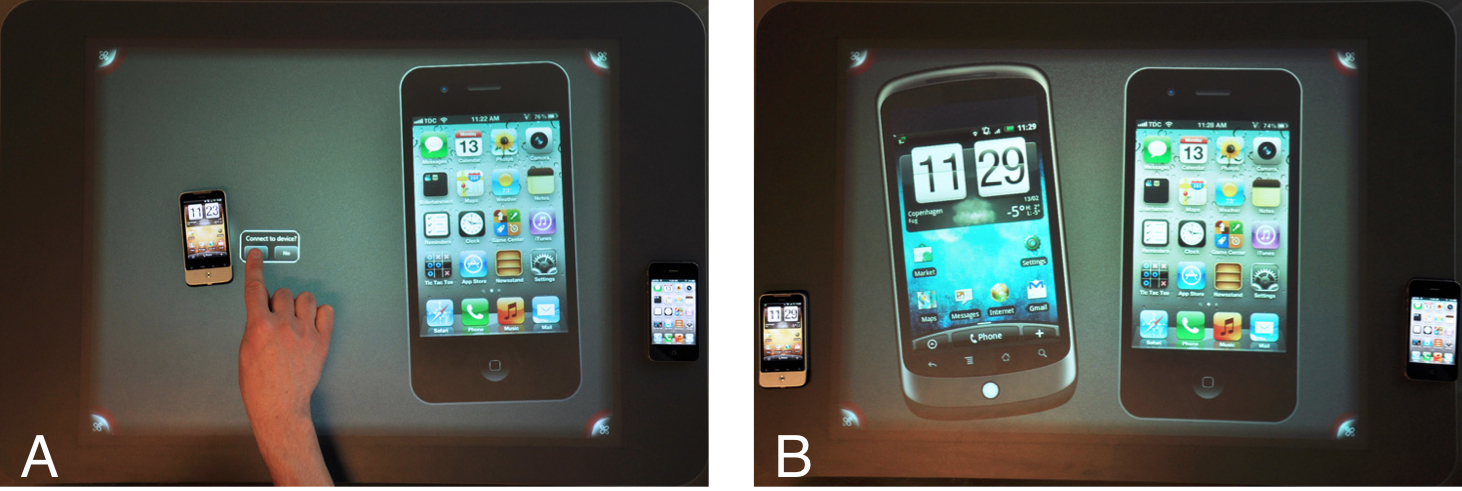
\includegraphics[width=0.7\linewidth]{images/sq2phones}
  \caption{(A) Pairing second device (B) Simultaneous devices}
  \label{fig:sq2phones}
\end{figure}

\subsection{Pairing}

The following design decisions address the requirements RA-1 to RA-4 (see p.~\pageref{RA}).

\begin{enumerate}[{DA}-1]
\item \hfill
	\begin{enumerate}[{DA-1}a]
	\item Pairing is triggered by placing the smartphone on the tabletop, as shown in figure~\ref{fig:sqPair}, for the reason that it is a simple gesture that is consistent with the form of the tabletop.
	\item Pairing is based on wireless connectivity, in order to provide spontaneity to the interaction.
	\end{enumerate}
	
\begin{figure}[htb]
  \centering
    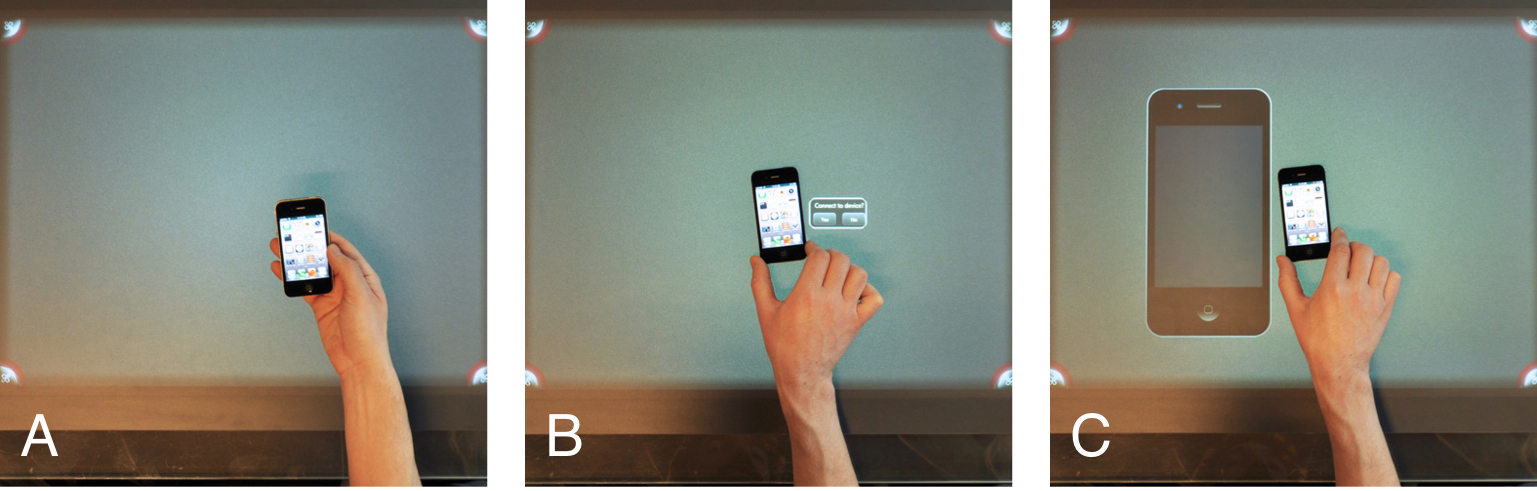
\includegraphics[width=0.7\linewidth]{images/sqPair}
  \caption{(A) Device in hand (B) Device detected (C) Device connected}
  \label{fig:sqPair}
\end{figure}

\item Device discovery relies on a standard networking protocol - in order to make it automatic, and provide spontaneity to the interaction.
\item The user must confirm the connection, both on the tabletop and on the smartphone, for reasons of security.
The tabletop should not be allowed to connect to an unknown device without explicit authorization, but the user should also be able to confirm that the smartphone is the correct one.
\item See DD-5.
\end{enumerate}

\subsection{Tracking}

The following design decisions address the requirements RB-1 to RB-4 (see p.~\pageref{RB}).

\label{DB}
\begin{enumerate}[{DB}-1]
\item Smartphones that come in contact with the tabletop are detected, using computer vision and shape recognition.
\item The location of the smartphones on the tabletop is tracked, using computer vision.
\item Removal of smartphones are detected using computer vision.
\item The replicated UI can be made active on the tabletop independently of the smartphone.
\end{enumerate}

\subsection{Replicated UI}

The following design decisions address the requirements RC-1 to RC-4 (see p.~\pageref{RC}).

\begin{enumerate}[{DC}-1]
\item The smartphone screen is replicated to the tabletop, using a standard desktop sharing protocol, for the reason that such protocols are platform independent and stable.
\item See DC-1.
\item See DC-1.
\item See DC-1.
\end{enumerate}

\subsection{Surface UI}

The following design decisions address the requirements RD-1 to RD-6 (see p.~\pageref{RD}).
It was decided to use multiple techniques to activate certain features.
The reason for this is to benefit from the advantages of all interaction techniques.
Some are easy to discover, and provide the learnability and intuitiveness that is looked for, while others are quicker and easier to use.
This is standard practice within software design, a good example being keyboard shortcuts, that are not easily discovered by a novice user, but are preferred by the expert user for their efficiency.

%\defaultlists
\label{DD}

\begin{enumerate}[{DD}-1]
\item The surface UI takes the form of an active border that contains the replicated UI, based on the user feedback.
It is a virtual replication of the physical body of the smartphone, to provide consistency in the user experience.
\item The replicated UI can be manipulated by using touch-based gestures on the surface UI, for reasons of consistency with both the smartphone and tabletop experiences.
	\begin{enumerate}[{DD-2}a]
	\item Dragging is done by performing a dragging gesture with one or more fingers.
	\item Rotating is done by
		\begin{enumerate}[1{.}]
		\item Dragging the corner of the surface UI, as shown in figure~\ref{fig:sq1f}

\begin{figure}[htb]
  \centering
    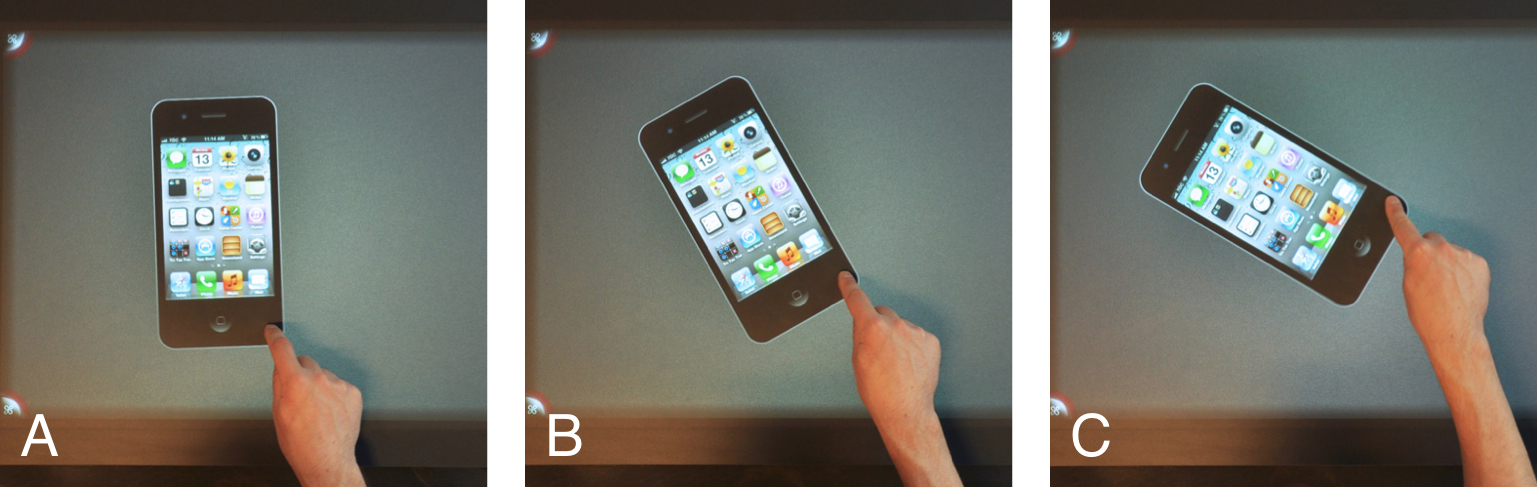
\includegraphics[width=0.7\linewidth]{images/sq1f}
  \caption{(A,B,C) Rotating using 1 finger.}
  \label{fig:sq1f}
\end{figure}

		\item Performing a rotating gesture with two fingers of the same hand, as shown in figure~\ref{fig:sq2f1h}

\begin{figure}[htb]
  \centering
    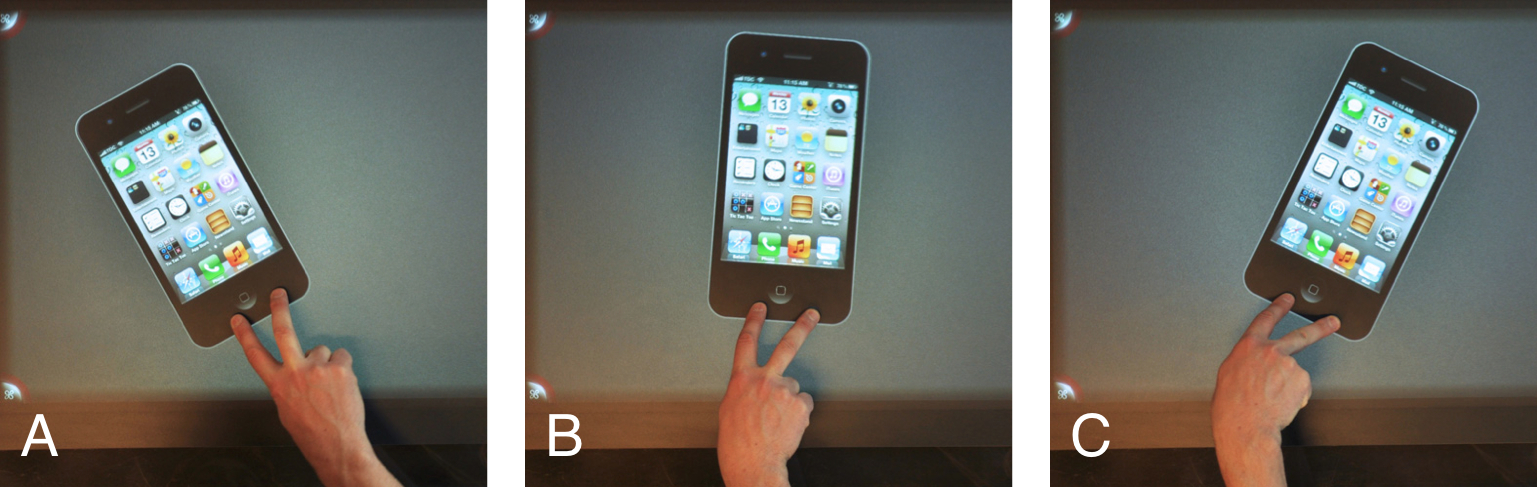
\includegraphics[width=0.7\linewidth]{images/sq2f1h}
  \caption{(A,B,C) Rotating using 2 fingers of the same hand.}
  \label{fig:sq2f1h}
\end{figure}

		\item Performing a rotating gesture with two hands
		\end{enumerate}
	\item Resizing is done by
		\begin{enumerate}[1{.}]
		\item Performing a pinching gesture with two fingers of the same hand
		\item Performing a resizing gesture with two hands, as shown in figure~\ref{fig:sqResize}
		
\begin{figure}[htb]
  \centering
    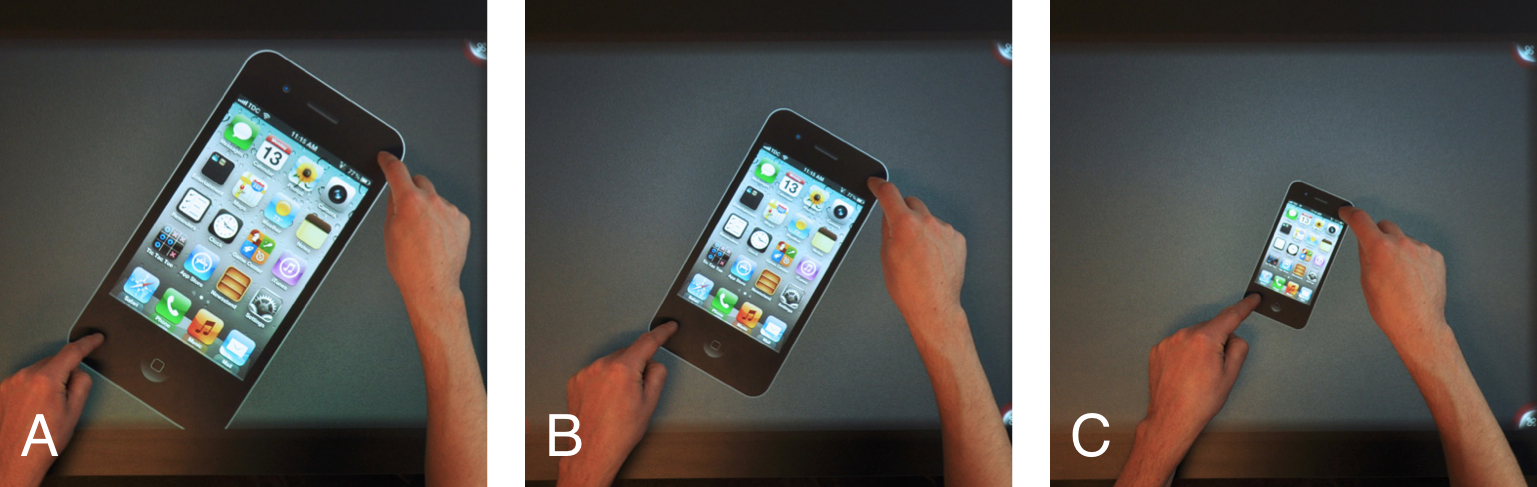
\includegraphics[width=0.7\linewidth]{images/sqResize}
  \caption{(A,B,C) Resizing down using both hands.}
  \label{fig:sqResize}
\end{figure}
		
		\end{enumerate}
	\end{enumerate}
\item Minimizing the replicated UI can be done by
	\begin{enumerate}[1{.}]
	\item Resizing the surface UI down
	\item Dragging the surface UI off an edge of the table, as shown in figure~\ref{fig:sqMin2}

\begin{figure}[htb]
  \centering
    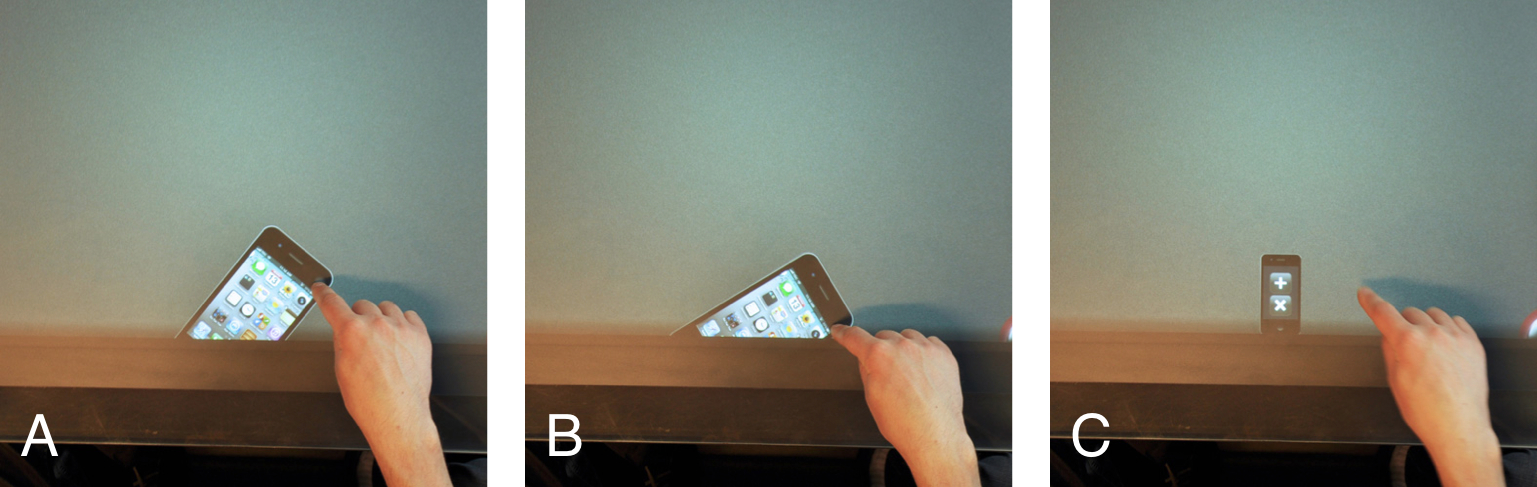
\includegraphics[width=0.7\linewidth]{images/sqMin2}
  \caption{(A,B,C) Minimizing by dragging off the edge.}
  \label{fig:sqMin2}
\end{figure}
	
	\item Double tapping the surface UI, as shown in figure~\ref{fig:sqMin1}
	\item Placing a full hand on the surface UI, as shown in figure~\ref{fig:sqMin1}
	\end{enumerate}
	
\begin{figure}[htb]
  \centering
    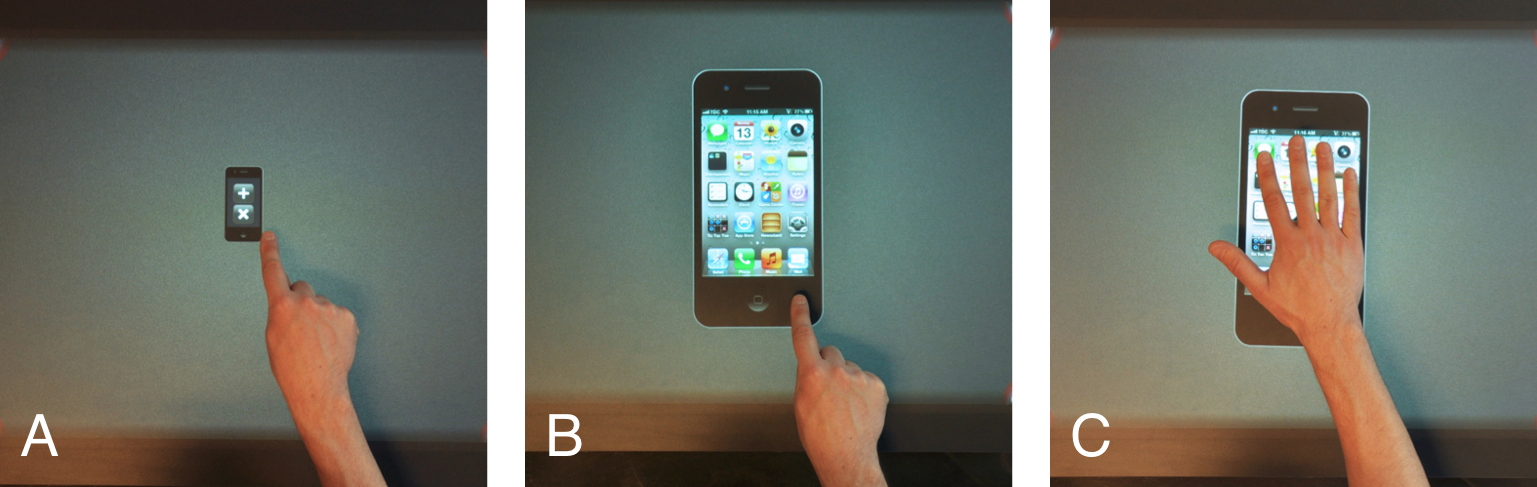
\includegraphics[width=0.7\linewidth]{images/sqMin1}
  \caption{(A) Minimized state (B) Double tap (C) Whole hand tap}
  \label{fig:sqMin1}
\end{figure}

When minimized, the surface UI appears as an icon on the tabletop, and can be restored by tapping a button.
\item Hiding the replicated UI is done by minimizing the surface UI, based on user feedback, see DC-3.
\item Closing the replicated UI is shown in figure~\ref{fig:sqClose}, it can be done by
	\begin{enumerate}[1{.}]
	\item Closing the minimized surface UI
	\item Dragging the surface UI to a corner of the tabletop
	\item Pressing and holding a finger on the active border
	\end{enumerate}

\begin{figure}[htb]
  \centering
    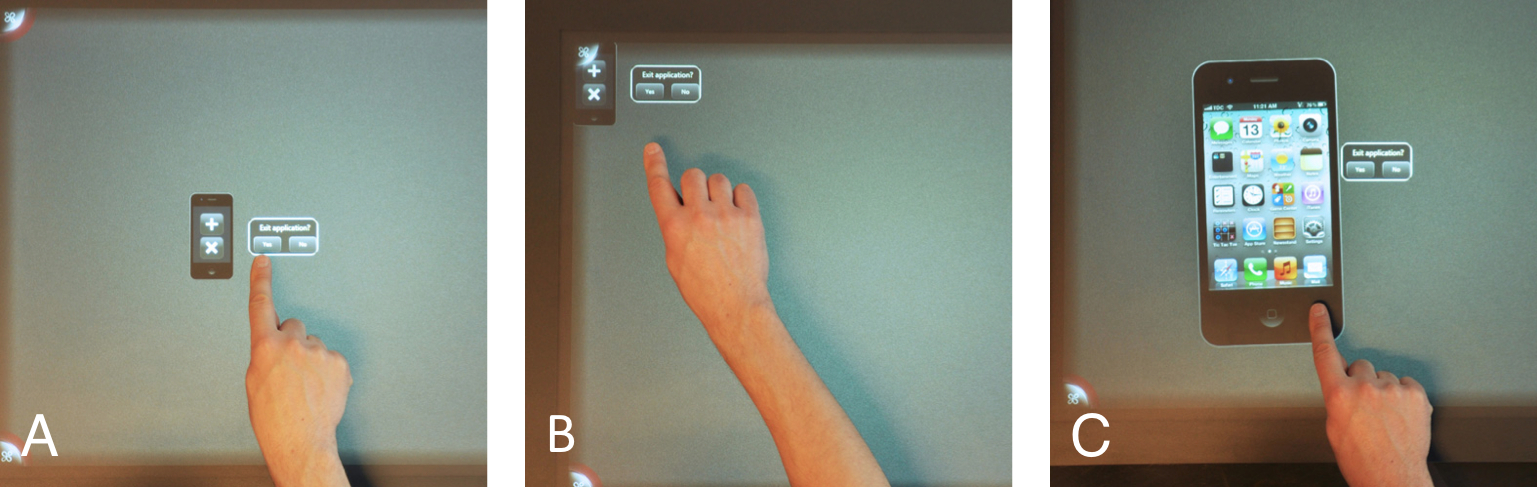
\includegraphics[width=0.7\linewidth]{images/sqClose}
  \caption{(A) Minimize then close (B) Close by dragging to a corner (C) Press and hold to close}
  \label{fig:sqClose}
\end{figure}

\item The functionalities provided by the smartphone's physical buttons can be accessed by tapping virtual replications of the buttons on the surface UI.
\end{enumerate}

\firmlists


